\section{M = 4--5 D}
\begin{center}
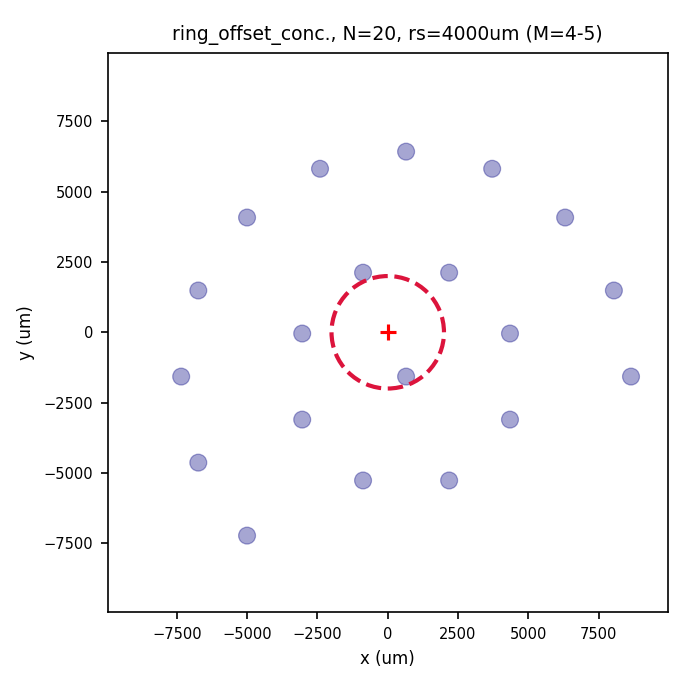
\includegraphics[width=0.55\textwidth]{winner_viz_figs/fig_M4_5.png}
\end{center}
\texttt{ring\_offset\_concentric}, ring\_spacing=4000\,$\mu$m, N=20,
a\_hole=600\,$\mu$m. Same geometry as M=2--3, smaller hole diameter (per the
acuity-optimal chart). Margin $+\infty$. Blind rate $\sim$10.5\%.

\section{M = 6 D, M = 8 D}
\begin{center}
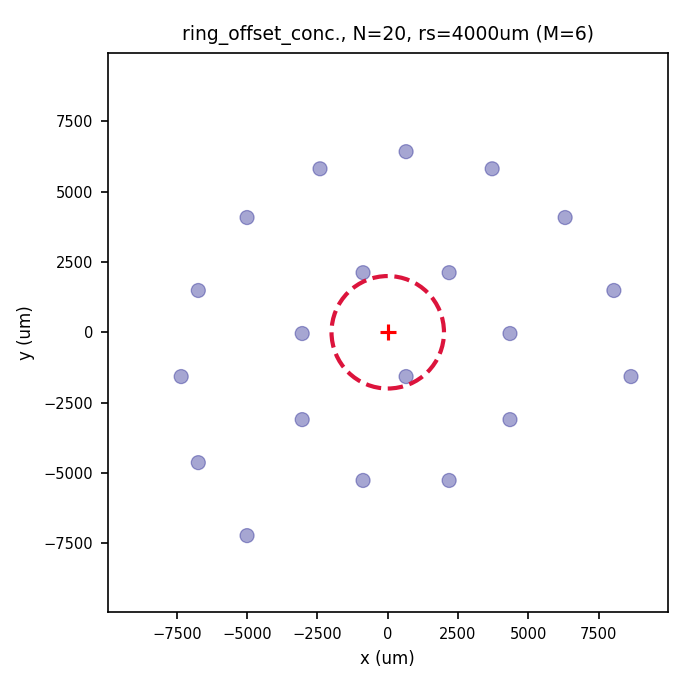
\includegraphics[width=0.55\textwidth]{winner_viz_figs/fig_M6.png}\quad
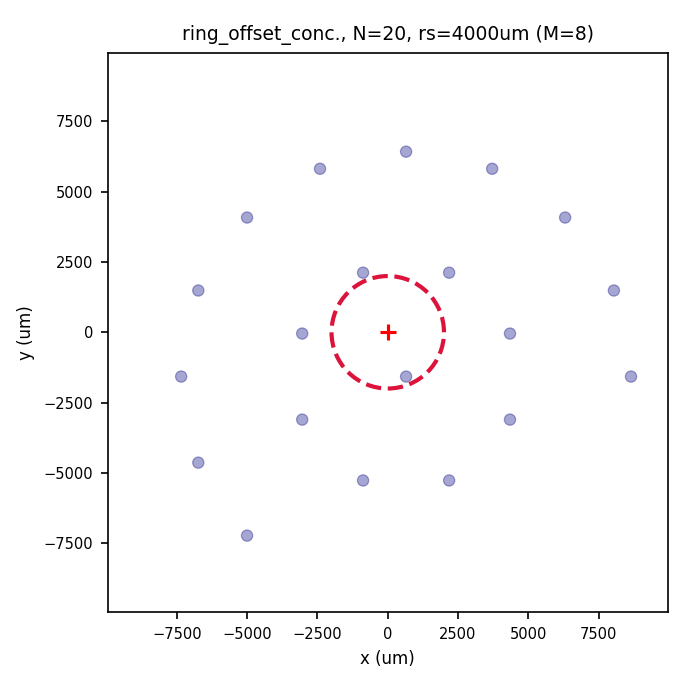
\includegraphics[width=0.55\textwidth]{winner_viz_figs/fig_M8.png}
\end{center}
Same \texttt{ring\_offset\_concentric} geometry again, a\_hole=500\,$\mu$m
(M=6, left) and 400\,$\mu$m (M=8, right). Margin $+\infty$ at both. Blind
rate 10.3\% and 10.1\% respectively.

\section{Global Scope (worst-case across all M)}
\begin{center}
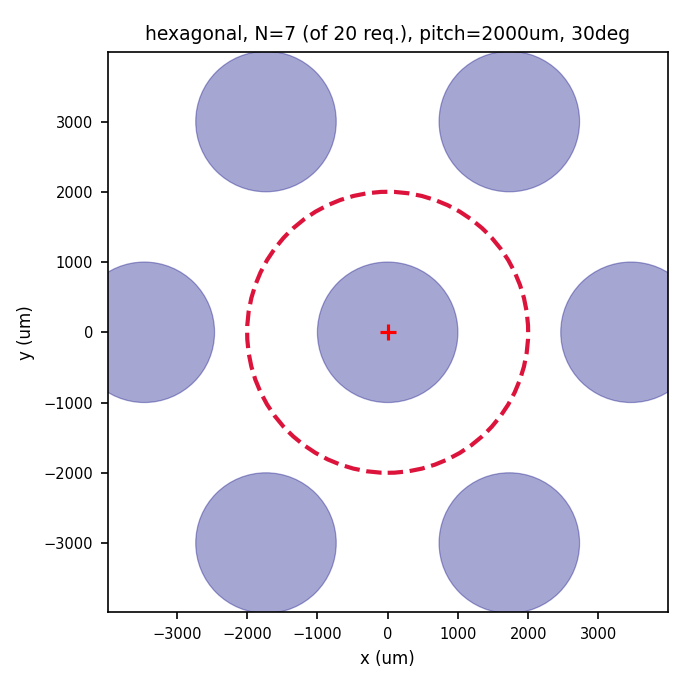
\includegraphics[width=0.55\textwidth]{winner_viz_figs/fig_global.png}
\end{center}
\texttt{hexagonal}, pitch=2000\,$\mu$m, rotation=30$^\circ$, N=7,
a\_hole=2000\,$\mu$m. Margin $+\infty$. Blind rate 17.3\%, the highest of any
winner --- the cost of guaranteeing safety across the full M=0--8D range with
one fixed geometry.

\newpage
